% mnras_template.tex
%
% LaTeX template for creating an MNRAS paper
%
% v3.0 released 14 May 2015
% (version numbers match those of mnras.cls)
%
% Copyright (C) Royal Astronomical Society 2015
% Authors:
% Keith T. Smith (Royal Astronomical Society)

% Change log
%
% v3.0 May 2015
%    Renamed to match the new package name
%    Version number matches mnras.cls
%    A few minor tweaks to wording
% v1.0 September 2013
%    Beta testing only - never publicly released
%    First version: a simple (ish) template for creating an MNRAS paper

%%%%%%%%%%%%%%%%%%%%%%%%%%%%%%%%%%%%%%%%%%%%%%%%%%
% Basic setup. Most papers should leave these options alone.
\documentclass[a4paper,fleqn,usenatbib]{mnras}

% MNRAS is set in Times font. If you don't have this installed (most LaTeX
% installations will be fine) or prefer the old Computer Modern fonts, comment
% out the following line
\usepackage{newtxtext,newtxmath}
% Depending on your LaTeX fonts installation, you might get better results with one of these:
%\usepackage{mathptmx}
%\usepackage{txfonts}

% Use vector fonts, so it zooms properly in on-screen viewing software
% Don't change these lines unless you know what you are doing
\usepackage[T1]{fontenc}
\usepackage{ae,aecompl}


%%%%% AUTHORS - PLACE YOUR OWN PACKAGES HERE %%%%%

% Only include extra packages if you really need them. Common packages are:
\usepackage{graphicx}	% Including figure files
\usepackage{amsmath}	% Advanced maths commands
\usepackage{amssymb}	% Extra maths symbols

%%%%%%%%%%%%%%%%%%%%%%%%%%%%%%%%%%%%%%%%%%%%%%%%%%

%%%%% AUTHORS - PLACE YOUR OWN COMMANDS HERE %%%%%

% Please keep new commands to a minimum, and use \newcommand not \def to avoid
% overwriting existing commands. Example:
%\newcommand{\pcm}{\,cm$^{-2}$}	% per cm-squared

\newcommand{\Msun}{\,\mathrm{M_{\sun}}}
\renewcommand{\labelenumi}{\arabic{enumi}. }

%%%%%%%%%%%%%%%%%%%%%%%%%%%%%%%%%%%%%%%%%%%%%%%%%%

%%%%%%%%%%%%%%%%%%% TITLE PAGE %%%%%%%%%%%%%%%%%%%

% Title of the paper, and the short title which is used in the headers.
% Keep the title short and informative.
\title[]{Insert clever, witty title here...}

% The list of authors, and the short list which is used in the headers.
% If you need two or more lines of authors, add an extra line using \newauthor
\author[I.D. Roberts \& L.C. Parker]{
Ian D. Roberts,\thanks{E-mail: roberid@mcmaster.ca}
Laura C. Parker
\\
% List of institutions
Department of Physics and Astronomy, McMaster University, Hamilton ON
L8S 4M1, Canada
}

% These dates will be filled out by the publisher
\date{Accepted XXX. Received YYY; in original form ZZZ}

% Enter the current year, for the copyright statements etc.
\pubyear{2016}

% Don't change these lines
\begin{document}
\label{firstpage}
\pagerange{\pageref{firstpage}--\pageref{lastpage}}
\maketitle

% Abstract of the paper
\begin{abstract}
\end{abstract}

% Select between one and six entries from the list of approved keywords.
% Don't make up new ones.
\begin{keywords}
galaxies: clusters: general -- galaxies: evolution -- galaxies:
groups: -- galaxies: statistics
\end{keywords}

%%%%%%%%%%%%%%%%%%%%%%%%%%%%%%%%%%%%%%%%%%%%%%%%%%

%%%%%%%%%%%%%%%%% BODY OF PAPER %%%%%%%%%%%%%%%%%%

\section{Introduction}
\label{sec:introduction}

%%%%%%%%%%%%%%%%%%%%%%%%%%%%%%%%%%%%%%%%

\section{Data}
\label{sec:data}

\subsection{Group sample}

For this work we employ the group catalogue of \citet{yang2007}, which
is constructed by applying the halo-based galaxy group finder from
\citet{yang2005, yang2007} to the New York University Value-Added
Galaxy Catalogue (NYU-VAGC; \citealt{blanton2005}).  The NYU-VAGC is a
low redshift galaxy catalogue (primarily $z \la 0.3$) consisting of
693319 galaxies derived from the Sloan Digital Sky Survey Data Release
7 (SDSS-DR7; \citealt{abazajian2009}).  We will briefly describe the
halo-based group finding algorithm used to generate the Yang group catalogue,
however for a more complete description the authors direct the reader
to \citet{yang2005} and \citet{yang2007}.
\par
First, the centres of potential groups are identified.  Galaxies are
initially assigned to groups using a traditional
``friends-of-friends'' (FOF) algorithm \citep[e.g.][]{huchra1982} with
very small linking lengths.  The luminosity-weighted centres 
FOF groups with at least two members are then taken as the centres of
potential groups and all galaxies not yet associated with a FOF group
are treated as tentative centres for potential groups.  A
characteristic luminosity, $L_{19.5}$, defined as the combined
luminosity of all group members with $^{0.1}M_r - 5\log h \le -19.5$,
is calculated for each tentative group and an initial halo mass is
assigned using an assumption for the group mass-to-light ratio,
$M_H/L_{19.5}$.  Utilizing this tentative group halo mass, velocity
dispersions and a virial radius are calculated for each group.  Next,
galaxies are assigned to groups under the assumption that the
distribution of galaxies in phase space follows that of dark matter
particles -- the distribution of dark matter particles is taken to
follow a spherical NFW profile \citep{navarro1997}.  Using the new
group memberships, group centres are recalculated and the procedure is
iterated until group memberships no longer change.
\par
We take group halo masses, $M_H$, from the Yang catalogue calculated
using a characteristic group stellar mass, $M_{\star,\text{grp}}$, and
assuming that there is a one-to-one relation between $M_{\star,\text{grp}}$
and $M_H$.  \citet{yang2007} define $M_{\star,\text{grp}}$ as

\begin{equation}
  M_{\star,\text{grp}} = \frac{1}{g(L_{19.5},\,L_{\text{lim}})} \sum_i
  \frac{M_{\star,i}}{\mathcal{C}_i}
\end{equation}

\noindent
where $M_{\star,i}$ is the stellar mass of the $i$th member galaxy,
$\mathcal{C}_i$ is the completeness of the survey at the position of
that galaxy, and $g(L_{19.5},\,L_{\text{lim}})$ is a correction factor
which accounts for galaxies missed due to the magnitude limit of the
survey.
\par
The Yang catalogue contains both haloes which would be broadly classified as
groups ($10^{12} \la M_H \la 10^{14}\Msun$) as well as clusters ($M_H
\ga 10^{14}\Msun$), however for brevity we will refer to all haloes as
groups regardless of halo mass unless otherwise specified.
\par
\textbf{(ADD GALAXY PROPERTIES INFORMATION)}

\subsection{Field sample}

For this research we also define a sample of ``field'' galaxies.  Like
the group sample, the field sample is also derived from the NYU-VAGC.
In order to construct the field sample we cross-match galaxies within
the Yang group catalogue against all galaxies within the NYU-VAGC
catalogue, and remove any galaxies which have been identified as being
members of Yang groups.  Furthermore, we apply an isolation
criteria and only keep galaxies which are separated from their
nearest-neighbour by a projected distance of at least
$0.5\,\mathrm{Mpc}$ and by at least $500\,\mathrm{km/s}$ in
line-of-sight velocity.

\subsection{Group dynamics}

\begin{figure}
  \centering
  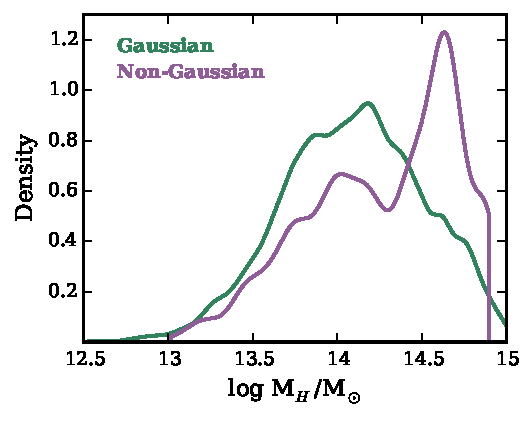
\includegraphics[width=\columnwidth]{mhdist_um.pdf}
  \caption{Smoothed host halo mass distributions for galaxies in the
    unmatched G and NG samples.}
  \label{fig:mhdist_um}
\end{figure}

To classify the dynamical state of the haloes in the data set we use a
combination of two statistical tests, the Anderson-Darling (AD)
normality test (\citealt{anderson1952}; see \citealt{hou2009, hou2013}
for an astronomical application) and the Dip test
(\citealt{hartigan1985}; see \citealt{ribeiro2013} for an astronomical
application).  The AD test is a non-parametric test of normality based
upon the comparison between the cumulative distribution function (CDF) of a
measured data sample and the CDF of a gaussian distribution.  Under
the assumption that the data is in fact normally distributed, the AD
test determines the probability ($p$) that the difference between
the CDFs of the data and a normal distribution equals or exceeds the
observed difference.  We apply the AD test to the velocity
distributions of the member galaxies of each group in the data sample,
thereby broadly classifying the dynamical state of each halo.  Our
first criteria in classifying a group as G is that the p-value given
by the AD test be greater than or equal to 0.05.  Our second criteria
required for a
group to be classified as G is that it be unimodal.  To specifically
gauge the modality of the velocity distribution of a given group we
use the Dip test.  Like the AD test, the Dip test is also a
non-parametric CDF statistic.  Where they differ is that the Dip test
looks for a flattening of the CDF for the data which would correspond
to a `dip' in the distribution being tested.  The Dip test operates
under the null hypothesis that the data is unimodal, and we consider a
group velocity distribution unimodal if the Dip test p-value is
greater than or equal to 0.05.  Therefore our G data sample consists
of all those groups with $p_{\text{ad}} \ge 0.05$
\emph{and} $p_{\text{dip}} \ge 0.05$, whereas our NG data
sample consists of all those groups with $p_{\text{ad}} < 0.05$
\emph{or} $p_{\text{dip}} < 0.05$.
\par
After applying the above criteria we find a G sample consisting of
42655 galaxies within 2447 groups and a NG sample consisting of 5306
galaxies within 215 groups.  The authors note that simply applying
these normality criteria in this fashion can lead to the NG sample
being biased toward rich, high halo mass groups (see
Fig.~\ref{fig:mhdist_um}).  To address this we
match of G and NG samples by halo mass (as well as stellar mass and
redshift), this matching procedure is laid out in the next section.

\subsection{Matched data set}

\begin{figure*}
  \centering
  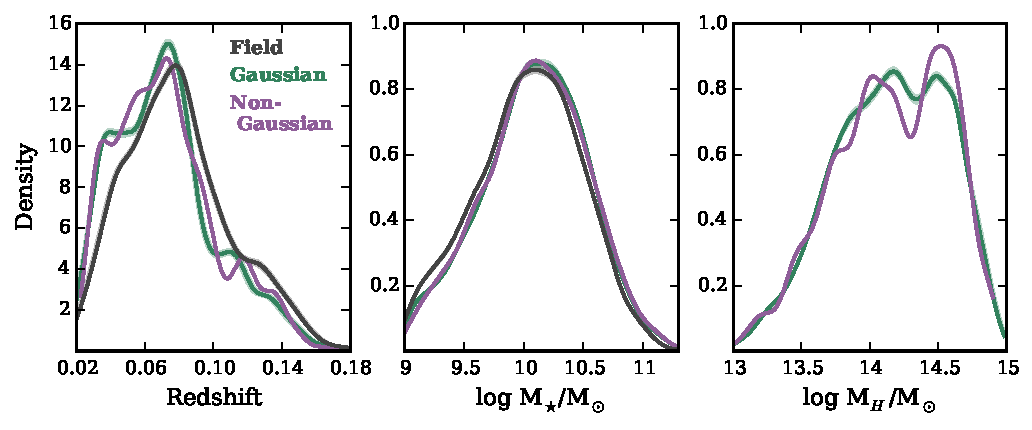
\includegraphics[width=\textwidth]{dist_m2_s.pdf}
  \caption{Smoothed distributions for stellar mass, redshift, and host
    halo mass for galaxies in the matched G, NG and field (where
    applicable) samples.  Shaded regions around the G and field lines
    are 90 per cent confidence intervals corresponding to the
    stochastic nature of our matching procedure.}
  \label{fig:dist_m2_s}
\end{figure*}

To ensure a fair comparison between galaxies in different environments
(ie.\ field galaxies, galaxies in G groups, and galaxies in NG groups)
we match our sample of G group galaxies and NG group galaxies by
stellar mass, redshift, and halo mass.  Additionally, we then match
our sample of field galaxies by stellar mass and redshift ensuring
that all of our galaxy samples are matched according to important galaxy
properties.  This is especially important when trying to elucidate
information on the effect of group dynamics on galaxy SF and
morphological properties for
two main reasons:
\par
First, stellar mass, redshift, and halo mass have
all been shown to influence galaxy SF and morphology
\citep[e.g.][]{brinchmann2004, feulner2005, zheng2007, cucciati2012, wetzel2012, lackner2013, tasca2014}; whereas
the impact of group dynamics is less clear \citep{hou2013, ribeiro2013} (REF) which is perhaps
suggestive of a more modest role.  Therefore,
if one hopes to identify trends in galaxy SF and morphology with group
dynamics it is crucial to properly control for these other effects.
\par
Second, standard statistical normality tests, such as the AD test, are
inherently biased in identifying non-Gaussian distributions when
sample size is large.  This is a result of the statistical power of
the test increasing with sample size which subsequently allows the
detection of more and more subtle departures from normality.  These subtle
departures from normality may not be physically relevant (in
principle, no group is truly Gaussian anyways) and what really matters is
whether galaxies in groups which show large departures from normality
have different properties than galaxies in groups which show smaller
departures from normality. Since group
richness generally scales with halo mass, in the absence of any matching
procedure, a sample of NG groups will be biased towards large halo
masses compared to a similar sample of G groups -- even though many
high halo mass NG groups may have been identified on the basis of very
small departures from normality.  Ensuring that our G and NG
samples have very similar halo mass distributions allows us to make a
fairer comparison between the two samples.
\par
Our algorithm for matching the G and NG samples is as follows:

\begin{enumerate}
  \item Our list of galaxies found in NG groups is iterated through,
    for each galaxy one `matching' galaxy from the G sample is
    found.  To be considered matching the two galaxies must have
    stellar masses within $0.1\,\mathrm{dex}$, redshifts within 0.01,
    and halo masses within $0.1\,\mathrm{dex}$.

  \item Step 1 is repeated continually until no more matches are
    found, the end result is a list of galaxies from the NG
    sample each of which will have one or more matching galaxies from
    the G sample assigned to them
  
  \item The matched G sample is generated by including two galaxies
    from the G sample for every one matching galaxy from the NG
    sample.  By definition this excludes any galaxies in the NG
    sample which only have one identified match.  However, 85 per cent
    of galaxies
    in the NG sample have two or more matches so although we reduce
    the NG sample size by 15 per cent it allows us to increase the
    matched G sample size twofold.

  \item In the case where a given galaxy in the NG sample has more
    than two identified matches, the two matching galaxies from the G sample are
    chosen randomly.  This introduces a stochastic nature to our
    analysis as each generation of the matched G sample will not
    contain exactly the same galaxies (although in each generation the
    G and NG samples will indeed be matched).  To account for this, any
    quantities calculated using the matched G sample are done so in a
    Monte Carlo sense where the median of 1000 stochastic generations
    is quoted along with 90 per cent confidence intervals.
\end{enumerate}

\noindent
The field sample is subsequently matched to the NG sample following
the same procedure, the same method is used to account for the
stochastic nature of the matching procedure.  Fig.~\ref{fig:dist_m2_s}
shows smoothed density
distributions of stellar mass, redshift, and halo mass for the matched
G, NG, and field samples.  Please note that for the remainder of the
paper all analysis is done using the matched samples, therefore from
this point forward any reference to the G or field samples is
implicitly referencing the matched samples.

%%%%%%%%%%%%%%%%%%%%%%%%%%%%%%%%%%%%%%%%%%%%

\section{Identifying infalling and virialized galaxies}
\label{sec:rad_div}

\begin{figure}
  \centering
  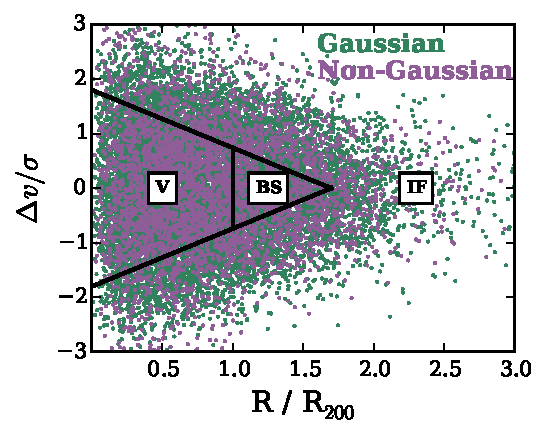
\includegraphics[width=\columnwidth]{vnorm_r.pdf}
  \caption{Velocity versus projected group-centric radius phase space
    for galaxies within the G and NG samples.  Virialized (C),
    backsplash (B), and infalling (A) regions from
    \citep{mahajan2011} are shown.}
  \label{fig:vnorm_r}
\end{figure}

Galaxies within group haloes can be broadly classified into three main
subclasses: galaxies infalling to the group at large radii, galaxies
virialized within the inner regions of the halo, and galaxies
backsplashing beyond the virial radius after making a passage through
the group centre.  In order to understand the radial dependence of
galaxy properties within groups \textbf{(REF)} it is crucial to be able to
identify these different galaxy populations
\citep{gill2005, mahajan2011, pimbblet2011}.
\par
The main focus of this paper is the comparison between the three
galaxy samples (field, G, NG) and to elucidate how the relationship
between these three samples evolves with the infall state of member
galaxies.  In particular we will compare star formation and
morphological properties for galaxies which are infalling into G and
NG groups to the same properties for galaxies which are virialized
within G and NG groups.
\par
One method used to distinguish between infalling, virialized, and
backsplash populations is to look for distinct populations in radial
phase space.  In particular \citet{mahajan2011} follow
\citet{sanchis2004} and identify galaxies within one virial radius as
virialized and use the cut

\begin{equation} \label{eq:cut}
  \frac{v_r}{V_\mathrm{v}} = -1.8 + 1.06
  \left(\frac{r}{R_\mathrm{v}}\right)
\end{equation}

\noindent
to distinguish between infalling and backsplash galaxies.  Where $v_r$
is the radial velocity of the galaxy, $V_\mathrm{v}$ is the velocity
dispersion of the group, $r$ is the group-centric radius, and
$R_\mathrm{v}$ is the virial radius of the group.
\par
The cuts described above were determined using full 6-d phase space
information, however observationally we are limited to line-of-sight
velocities and projected radii.  Although working in projection
removes much of the distinct phase space structure \citep{oman2013},
density contours for the virialized, backsplash, and infalling
populations still occupy similar regions in projected phase space
with the contamination between different populations being more substantial
\citep{mahajan2011}.  While the divisions between populations is
certainly less clear in projection, equation~\ref{eq:cut} can still be
used to obtain an approximate division between infalling, virialized,
and backsplash galaxies -- this approximation is preferred over
the incorrect assumption that all galaxies beyond the virial radius
are infalling for the first time.
\par
To make the transformation to observational quantities we replace
$v_r/V_\mathrm{v}$ with $\Delta cz/\sigma$ and $r/R_\mathrm{v}$ with
$R/R_{200}$ in equation~\ref{eq:cut}.  We also symmetrize the phase
space cuts to account for projection by using the mirror of
equation~\ref{eq:cut}.  After implementing these observational
adjustments, and utilizing the best-fitting scheme from
\citet{mahajan2011}, we are able to plot in Fig.~\ref{fig:vnorm_r} the
phase space distribution of galaxies within the G and NG samples
divided into the infalling (Regions A), backsplash (Region B), and
virialized (Region C) populations. 

%%%%%%%%%%%%%%%%%%%%%%%%%%%%%%%%%%%%%%%%%%%%

\section{Galaxy properties in the infall region}
\label{sec:infall}

\begin{figure*}
  \centering
  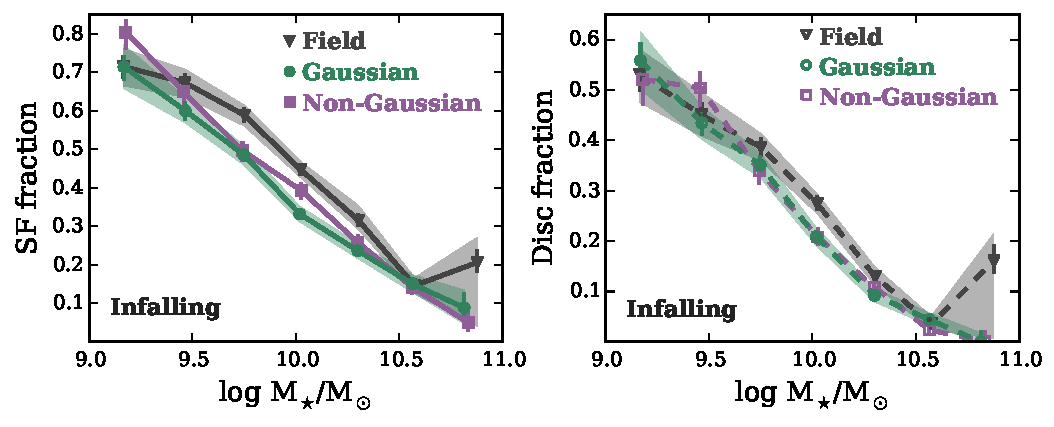
\includegraphics[width=\textwidth]{disk_sfFrac_w2_if.pdf}
  \caption{Star forming and disc fraction versus stellar mass for
    field galaxies as well as infalling galaxies in the G and NG
    samples.  Error bars correspond to $1 \sigma$ binomial confidence
    intervals as given in \citet{cameron2011}, shaded regions are 90
    per cent Monte Carlo confidence intervals derived from the
    stochastic nature of the matching procedure.}
  \label{fig:disk_sfFrac_if}
\end{figure*}

\begin{figure}
  \centering
  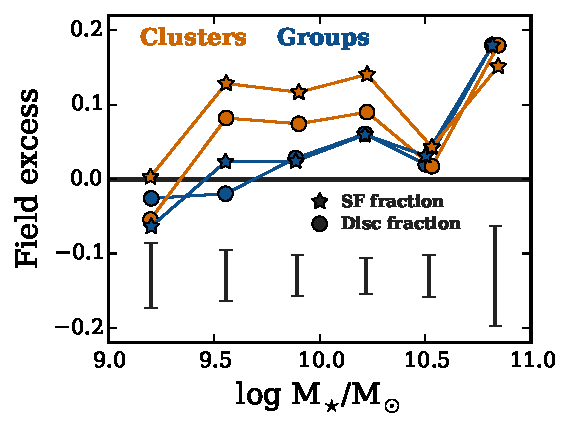
\includegraphics[width=\columnwidth]{mh_excess.pdf}
  \caption{Field excess versus stellar mass for galaxies within groups
  ($10^{12} < M_H < 10^{14} \Msun$) and clusters ($M_H \ge 10^{14}
    \Msun$).  Mean $1 \sigma$ error bars are shown for each bin.}
  \label{fig:mh_excess}
\end{figure}

%%%%%%%%%%%%%%%%%%%%%%%%%%%%%%%%%%%%%%%%%%%%%%

\section{Galaxy properties in the virialized region}
\label{sec:virial}

\begin{figure*}
  \centering
  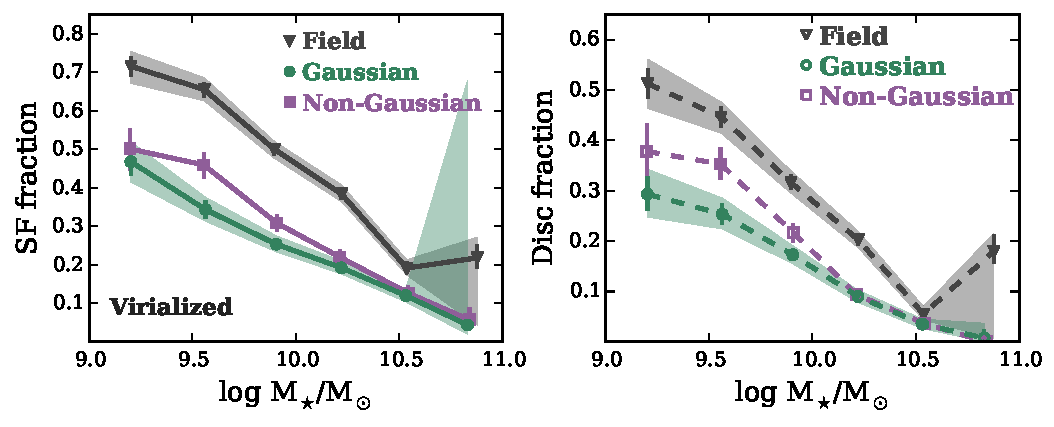
\includegraphics[width=\textwidth]{disk_sfFrac_w2_v.pdf}
  \caption{Star forming and disc fraction versus stellar mass for
    field galaxies as well as virialized galaxies in the G and NG
    samples.  Error bars correspond to $1 \sigma$ binomial confidence
    intervals as given in \citet{cameron2011}, shaded regions are 90
    per cent Monte Carlo confidence intervals derived from the
    stochastic nature of the matching procedure.}
  \label{fig:disk_sfFrac_v}
\end{figure*}

%%%%%%%%%%%%%%%%%%%%%%%%%%%%%%%%%%%%%%%%%%%

\section{Discussion}
\label{sec:discussion}

%%%%%%%%%%%%%%%%%%%%%%%%%%%%%%%%%%%%%%%%%%%

\section{Summary \& conclusions}
\label{sec:summary} 

%%%%%%%%%%%%%%%%%%%%%%%%%%%%%%%%%%%%%%%%%%

\section*{Acknowledgments}
\label{sec:acknowledgments}

IDR thanks the Ontario Graduate Scholarship program for funding.  LCP
thanks the National Science and Engineering Research
Council of Canada for funding.  The authors thank
F. Evans for matching together the various SDSS catalogues used in
this research.  We thank X. Yang et al. for
making their
SDSS DR7 group catalogue publicly available, L. Simard et al. for the
publication of their SDSS DR7 morphology catalogue, J. Brinchmann et al. for
publication of their SDSS SFRs, and the NYU-VAGC
team for the 
publication of their SDSS DR7 catalogue.  This research would not have
been possible without access to these public catalogues.
\par
Funding for the SDSS has been provided by the Alfred P. Sloan
Foundation, the Participating Institutions, the National Science
Foundation, the U.S. Department of Energy, the National Aeronautics
and Space Administration, the Japanese Monbukagakusho, the Max Planck
Society, and the Higher Education Funding Council for England. The
SDSS Web Site is http://www.sdss.org/.
\par
The SDSS is managed by the Astrophysical Research Consortium for the
Participating Institutions. The Participating Institutions are the
American Museum of Natural History, Astrophysical Institute Potsdam,
University of Basel, University of Cambridge, Case Western Reserve
University, University of Chicago, Drexel University, Fermilab, the
Institute for Advanced Study, the Japan Participation Group, Johns
Hopkins University, the Joint Institute for Nuclear Astrophysics, the
Kavli Institute for Particle Astrophysics and Cosmology, the Korean
Scientist Group, the Chinese Academy of Sciences (LAMOST), Los Alamos
National Laboratory, the Max-Planck-Institute for Astronomy (MPIA),
the Max-Planck-Institute for Astrophysics (MPA), New Mexico State
University, Ohio State University, University of Pittsburgh,
University of Portsmouth, Princeton University, the United States
Naval Observatory, and the University of Washington.

%%%%%%%%%%%%%%%%%%%%%%%%%%%%%%%%%%%%%%%%%%%%%%%%%%

%%%%%%%%%%%%%%%%%%%% REFERENCES %%%%%%%%%%%%%%%%%%

% The best way to enter references is to use BibTeX:

\bibliographystyle{mnras}
\bibliography{RobertsParker2016} % if your bibtex file is called example.bib


% Alternatively you could enter them by hand, like this:
% This method is tedious and prone to error if you have lots of references
%\begin{thebibliography}{99}
%\bibitem[\protect\citeauthoryear{Author}{2012}]{Author2012}
%Author A.~N., 2013, Journal of Improbable Astronomy, 1, 1
%\bibitem[\protect\citeauthoryear{Others}{2013}]{Others2013}
%Others S., 2012, Journal of Interesting Stuff, 17, 198
%\end{thebibliography}


% Don't change these lines
\bsp	% typesetting comment
\label{lastpage}
\end{document}

% End of mnras_template.tex
